\chapter{Question 3}
\assignment{
        Formulate stability of linear switched system with a common quadratic Lyapunov function. Give an example
}
If we say we have multiple linear systems for which we are switching arbitrary between.

\begin{equation}
        \dot{x} = Ax \quad \rightarrow \quad
        \begin{Bmatrix}
                \dot{x} = A_1 x \\
                \vdots \\
                \dot{x} = A_i x
        \end{Bmatrix}
\end{equation}
We can formulate a necessary condition for AS; which is that for every system in the switching system should be Hurwitz.

Even though all the systems is asymptotically stable it would still be possible to construct a divergent trajectory from any initial state, except for some special cases where $A_i$ is pairwise commutative ($A_iA_j = A_j A_i$, for all $i,j \in I$) or symmetric ($A_i = A_i^T$ for all $i$), or $A_i$ is normal ($A_iA_i^T = A_i^T A_i$ for all $i$).

An other way to formulate stability of linear switched systems is to find a common quadratic Lyapunov function (CQLF) for all the systems in the switching system.

\begin{equation}
        \begin{split}
                V(x) &= x^T P x \geq 0 \quad \forall \quad D \\
                \dot{V}(x) &= \frac{\partial V}{\partial x} f(x) < 0 \quad \forall \quad D - <0> \\
                V(0) &= 0
        \end{split}
\end{equation}
The conditions for the existence of a CQLF can be expressed as an LMI, namely the existance of a symmetric matrix $P$,$P \in \mathbb{R}^{n\times n}$ such that:
\begin{equation}
        P > 0, \quad PA_i + A_i^TP < 0, \quad \forall i \in I
\end{equation}

\begin{figure}[htbp]
        \centering
        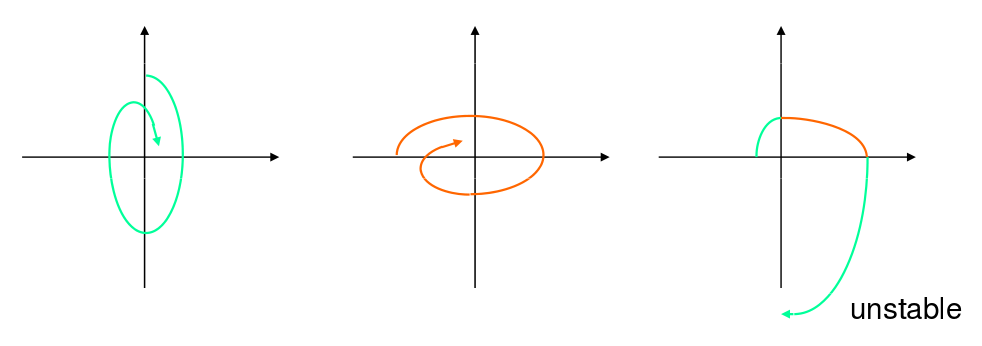
\includegraphics[width=0.8\textwidth]{switching_systems.png}
        \caption{Shows that asymptotic stability for each subsystem is necessary but not sufficient.}
        \label{fig:switching_systems}
\end{figure}